% Options for packages loaded elsewhere
\PassOptionsToPackage{unicode}{hyperref}
\PassOptionsToPackage{hyphens}{url}
%
\documentclass[
]{article}
\usepackage{amsmath,amssymb}
\usepackage{lmodern}
\usepackage{ifxetex,ifluatex}
\ifnum 0\ifxetex 1\fi\ifluatex 1\fi=0 % if pdftex
  \usepackage[T1]{fontenc}
  \usepackage[utf8]{inputenc}
  \usepackage{textcomp} % provide euro and other symbols
\else % if luatex or xetex
  \usepackage{unicode-math}
  \defaultfontfeatures{Scale=MatchLowercase}
  \defaultfontfeatures[\rmfamily]{Ligatures=TeX,Scale=1}
\fi
% Use upquote if available, for straight quotes in verbatim environments
\IfFileExists{upquote.sty}{\usepackage{upquote}}{}
\IfFileExists{microtype.sty}{% use microtype if available
  \usepackage[]{microtype}
  \UseMicrotypeSet[protrusion]{basicmath} % disable protrusion for tt fonts
}{}
\makeatletter
\@ifundefined{KOMAClassName}{% if non-KOMA class
  \IfFileExists{parskip.sty}{%
    \usepackage{parskip}
  }{% else
    \setlength{\parindent}{0pt}
    \setlength{\parskip}{6pt plus 2pt minus 1pt}}
}{% if KOMA class
  \KOMAoptions{parskip=half}}
\makeatother
\usepackage{xcolor}
\IfFileExists{xurl.sty}{\usepackage{xurl}}{} % add URL line breaks if available
\IfFileExists{bookmark.sty}{\usepackage{bookmark}}{\usepackage{hyperref}}
\hypersetup{
  pdftitle={compgen2021: Week 1 exercises},
  pdfauthor={O. Daniel López Olmos},
  hidelinks,
  pdfcreator={LaTeX via pandoc}}
\urlstyle{same} % disable monospaced font for URLs
\usepackage[margin=1in]{geometry}
\usepackage{color}
\usepackage{fancyvrb}
\newcommand{\VerbBar}{|}
\newcommand{\VERB}{\Verb[commandchars=\\\{\}]}
\DefineVerbatimEnvironment{Highlighting}{Verbatim}{commandchars=\\\{\}}
% Add ',fontsize=\small' for more characters per line
\usepackage{framed}
\definecolor{shadecolor}{RGB}{248,248,248}
\newenvironment{Shaded}{\begin{snugshade}}{\end{snugshade}}
\newcommand{\AlertTok}[1]{\textcolor[rgb]{0.94,0.16,0.16}{#1}}
\newcommand{\AnnotationTok}[1]{\textcolor[rgb]{0.56,0.35,0.01}{\textbf{\textit{#1}}}}
\newcommand{\AttributeTok}[1]{\textcolor[rgb]{0.77,0.63,0.00}{#1}}
\newcommand{\BaseNTok}[1]{\textcolor[rgb]{0.00,0.00,0.81}{#1}}
\newcommand{\BuiltInTok}[1]{#1}
\newcommand{\CharTok}[1]{\textcolor[rgb]{0.31,0.60,0.02}{#1}}
\newcommand{\CommentTok}[1]{\textcolor[rgb]{0.56,0.35,0.01}{\textit{#1}}}
\newcommand{\CommentVarTok}[1]{\textcolor[rgb]{0.56,0.35,0.01}{\textbf{\textit{#1}}}}
\newcommand{\ConstantTok}[1]{\textcolor[rgb]{0.00,0.00,0.00}{#1}}
\newcommand{\ControlFlowTok}[1]{\textcolor[rgb]{0.13,0.29,0.53}{\textbf{#1}}}
\newcommand{\DataTypeTok}[1]{\textcolor[rgb]{0.13,0.29,0.53}{#1}}
\newcommand{\DecValTok}[1]{\textcolor[rgb]{0.00,0.00,0.81}{#1}}
\newcommand{\DocumentationTok}[1]{\textcolor[rgb]{0.56,0.35,0.01}{\textbf{\textit{#1}}}}
\newcommand{\ErrorTok}[1]{\textcolor[rgb]{0.64,0.00,0.00}{\textbf{#1}}}
\newcommand{\ExtensionTok}[1]{#1}
\newcommand{\FloatTok}[1]{\textcolor[rgb]{0.00,0.00,0.81}{#1}}
\newcommand{\FunctionTok}[1]{\textcolor[rgb]{0.00,0.00,0.00}{#1}}
\newcommand{\ImportTok}[1]{#1}
\newcommand{\InformationTok}[1]{\textcolor[rgb]{0.56,0.35,0.01}{\textbf{\textit{#1}}}}
\newcommand{\KeywordTok}[1]{\textcolor[rgb]{0.13,0.29,0.53}{\textbf{#1}}}
\newcommand{\NormalTok}[1]{#1}
\newcommand{\OperatorTok}[1]{\textcolor[rgb]{0.81,0.36,0.00}{\textbf{#1}}}
\newcommand{\OtherTok}[1]{\textcolor[rgb]{0.56,0.35,0.01}{#1}}
\newcommand{\PreprocessorTok}[1]{\textcolor[rgb]{0.56,0.35,0.01}{\textit{#1}}}
\newcommand{\RegionMarkerTok}[1]{#1}
\newcommand{\SpecialCharTok}[1]{\textcolor[rgb]{0.00,0.00,0.00}{#1}}
\newcommand{\SpecialStringTok}[1]{\textcolor[rgb]{0.31,0.60,0.02}{#1}}
\newcommand{\StringTok}[1]{\textcolor[rgb]{0.31,0.60,0.02}{#1}}
\newcommand{\VariableTok}[1]{\textcolor[rgb]{0.00,0.00,0.00}{#1}}
\newcommand{\VerbatimStringTok}[1]{\textcolor[rgb]{0.31,0.60,0.02}{#1}}
\newcommand{\WarningTok}[1]{\textcolor[rgb]{0.56,0.35,0.01}{\textbf{\textit{#1}}}}
\usepackage{graphicx}
\makeatletter
\def\maxwidth{\ifdim\Gin@nat@width>\linewidth\linewidth\else\Gin@nat@width\fi}
\def\maxheight{\ifdim\Gin@nat@height>\textheight\textheight\else\Gin@nat@height\fi}
\makeatother
% Scale images if necessary, so that they will not overflow the page
% margins by default, and it is still possible to overwrite the defaults
% using explicit options in \includegraphics[width, height, ...]{}
\setkeys{Gin}{width=\maxwidth,height=\maxheight,keepaspectratio}
% Set default figure placement to htbp
\makeatletter
\def\fps@figure{htbp}
\makeatother
\setlength{\emergencystretch}{3em} % prevent overfull lines
\providecommand{\tightlist}{%
  \setlength{\itemsep}{0pt}\setlength{\parskip}{0pt}}
\setcounter{secnumdepth}{-\maxdimen} % remove section numbering
\ifluatex
  \usepackage{selnolig}  % disable illegal ligatures
\fi

\title{compgen2021: Week 1 exercises}
\author{O. Daniel López Olmos}
\date{}

\begin{document}
\maketitle

\hypertarget{exercises-for-week1}{%
\section{Exercises for Week1}\label{exercises-for-week1}}

\hypertarget{statistics-for-genomics}{%
\subsection{Statistics for genomics}\label{statistics-for-genomics}}

\hypertarget{how-to-summarize-collection-of-data-points-the-idea-behind-statistical-distributions}{%
\subsubsection{How to summarize collection of data points: The idea
behind statistical
distributions}\label{how-to-summarize-collection-of-data-points-the-idea-behind-statistical-distributions}}

\begin{enumerate}
\def\labelenumi{\arabic{enumi}.}
\tightlist
\item
  Calculate the means and variances of the rows of the following
  simulated data set, and plot the distributions of means and variances
  using \texttt{hist()} and \texttt{boxplot()} functions. {[}Difficulty:
  \textbf{Beginner/Intermediate}{]}
\end{enumerate}

\begin{Shaded}
\begin{Highlighting}[]
\CommentTok{\#import libraries}
\FunctionTok{library}\NormalTok{(mosaic, }\AttributeTok{warn.conflicts =}\NormalTok{ F)}
\end{Highlighting}
\end{Shaded}

\begin{verbatim}
## Registered S3 method overwritten by 'mosaic':
##   method                           from   
##   fortify.SpatialPolygonsDataFrame ggplot2
\end{verbatim}

\begin{verbatim}
## 
## The 'mosaic' package masks several functions from core packages in order to add 
## additional features.  The original behavior of these functions should not be affected by this.
\end{verbatim}

\begin{Shaded}
\begin{Highlighting}[]
\FunctionTok{set.seed}\NormalTok{(}\DecValTok{100}\NormalTok{)}

\CommentTok{\#sample data matrix from normal distribution}
\NormalTok{gset}\OtherTok{=}\FunctionTok{rnorm}\NormalTok{(}\DecValTok{600}\NormalTok{,}\AttributeTok{mean=}\DecValTok{200}\NormalTok{,}\AttributeTok{sd=}\DecValTok{70}\NormalTok{)}
\NormalTok{data}\OtherTok{=}\FunctionTok{matrix}\NormalTok{(gset,}\AttributeTok{ncol=}\DecValTok{6}\NormalTok{)}

\CommentTok{\#calculate means and variances }
\NormalTok{rowMeans }\OtherTok{\textless{}{-}} \FunctionTok{apply}\NormalTok{(data, }\DecValTok{1}\NormalTok{, mean)}
\NormalTok{rowVars }\OtherTok{\textless{}{-}} \FunctionTok{apply}\NormalTok{(data, }\DecValTok{1}\NormalTok{, var)}

\CommentTok{\#plot the distributions}
\FunctionTok{hist}\NormalTok{(rowMeans, }\AttributeTok{col =} \StringTok{"lightblue"}\NormalTok{, }\AttributeTok{border =} \StringTok{"white"}\NormalTok{,}
     \AttributeTok{main =} \StringTok{"Distribution of the means calculated row{-}wise"}\NormalTok{,}
     \AttributeTok{xlab =} \StringTok{"Row means"}\NormalTok{)}
\end{Highlighting}
\end{Shaded}

\includegraphics{week1_exercises_files/figure-latex/getDataChp3Ex-1.pdf}

\begin{Shaded}
\begin{Highlighting}[]
\FunctionTok{hist}\NormalTok{(rowVars, }\AttributeTok{col =} \StringTok{"lightblue"}\NormalTok{, }\AttributeTok{border =} \StringTok{"white"}\NormalTok{,}
     \AttributeTok{main =} \StringTok{"Distribution of the variances calculated row{-}wise"}\NormalTok{,}
     \AttributeTok{xlab =} \StringTok{"Row variances"}\NormalTok{)}
\end{Highlighting}
\end{Shaded}

\includegraphics{week1_exercises_files/figure-latex/getDataChp3Ex-2.pdf}

\begin{enumerate}
\def\labelenumi{\arabic{enumi}.}
\setcounter{enumi}{1}
\item
  Using the data generated above, calculate the standard deviation of
  the distribution of the means using the \texttt{sd()} function.
  Compare that to the expected standard error obtained from the central
  limit theorem keeping in mind the population parameters were
  \(\sigma=70\) and \(n=6\). How does the estimate from the random
  samples change if we simulate more data with
  \texttt{data=matrix(rnorm(6000,mean=200,sd=70),ncol=6)}?
  {[}Difficulty: \textbf{Beginner/Intermediate}{]}
\item
  Simulate 30 random variables using the \texttt{rpois()} function. Do
  this 1000 times and calculate the mean of each sample. Plot the
  sampling distributions of the means using a histogram. Get the 2.5th
  and 97.5th percentiles of the distribution. {[}Difficulty:
  \textbf{Beginner/Intermediate}{]}
\end{enumerate}

\begin{Shaded}
\begin{Highlighting}[]
\FunctionTok{require}\NormalTok{(mosaic, }\AttributeTok{quietly =}\NormalTok{ T)}
\CommentTok{\#HINT}
\FunctionTok{set.seed}\NormalTok{(}\DecValTok{100}\NormalTok{)}

\CommentTok{\#sample 30 values from poisson dist with lambda paramater = 30}
\NormalTok{pois1 }\OtherTok{\textless{}{-}} \FunctionTok{rpois}\NormalTok{(}\DecValTok{30}\NormalTok{, }\AttributeTok{lambda=}\DecValTok{5}\NormalTok{)}
\CommentTok{\#bootstrap resampling}
\NormalTok{bootMeans }\OtherTok{=}\NormalTok{ mosaic}\SpecialCharTok{::}\FunctionTok{do}\NormalTok{(}\DecValTok{1000}\NormalTok{) }\SpecialCharTok{*} \FunctionTok{mean}\NormalTok{(}\FunctionTok{resample}\NormalTok{(pois1))}
\CommentTok{\#get percentiles from the bootstrap means}
\NormalTok{q }\OtherTok{=} \FunctionTok{quantile}\NormalTok{(bootMeans[, }\DecValTok{1}\NormalTok{], }\AttributeTok{p =} \FunctionTok{c}\NormalTok{(}\FloatTok{0.025}\NormalTok{, }\FloatTok{0.975}\NormalTok{))}

\CommentTok{\#plot sampling distributions}
\FunctionTok{hist}\NormalTok{(bootMeans[,}\DecValTok{1}\NormalTok{], }\AttributeTok{col =} \StringTok{"lightblue"}\NormalTok{, }\AttributeTok{border =} \StringTok{"white"}\NormalTok{,}
                    \AttributeTok{xlab =} \StringTok{"Sample means"}\NormalTok{)}
\FunctionTok{abline}\NormalTok{(}\AttributeTok{v =} \FunctionTok{c}\NormalTok{(q[}\DecValTok{1}\NormalTok{], q[}\DecValTok{2}\NormalTok{] ), }\AttributeTok{col =} \StringTok{"black"}\NormalTok{)}
\FunctionTok{text}\NormalTok{(}\AttributeTok{x =}\NormalTok{ q[}\DecValTok{1}\NormalTok{], }\AttributeTok{y =} \DecValTok{200}\NormalTok{, }\FunctionTok{round}\NormalTok{(q[}\DecValTok{1}\NormalTok{], }\DecValTok{3}\NormalTok{), }\AttributeTok{adj =} \FunctionTok{c}\NormalTok{(}\DecValTok{1}\NormalTok{, }\DecValTok{0}\NormalTok{))}
\FunctionTok{text}\NormalTok{(}\AttributeTok{x =}\NormalTok{ q[}\DecValTok{2}\NormalTok{], }\AttributeTok{y =} \DecValTok{200}\NormalTok{, }\FunctionTok{round}\NormalTok{(q[}\DecValTok{2}\NormalTok{], }\DecValTok{3}\NormalTok{), }\AttributeTok{adj =} \FunctionTok{c}\NormalTok{(}\DecValTok{0}\NormalTok{, }\DecValTok{0}\NormalTok{))}
\end{Highlighting}
\end{Shaded}

\includegraphics{week1_exercises_files/figure-latex/exRpoisChp3-1.pdf}
4. Use the \texttt{t.test()} function to calculate confidence intervals
of the mean on the first random sample \texttt{pois1} simulated from the
\texttt{rpois()} function below. {[}Difficulty: \textbf{Intermediate}{]}

\begin{Shaded}
\begin{Highlighting}[]
\CommentTok{\#calculate confidence intervals with \textquotesingle{}t.test()\textquotesingle{}}
\FunctionTok{t.test}\NormalTok{(pois1)}
\end{Highlighting}
\end{Shaded}

\begin{verbatim}
## 
##  One Sample t-test
## 
## data:  pois1
## t = 17.663, df = 29, p-value < 2.2e-16
## alternative hypothesis: true mean is not equal to 0
## 95 percent confidence interval:
##  4.362104 5.504563
## sample estimates:
## mean of x 
##  4.933333
\end{verbatim}

Confidence intervals: {[}4.362104, 5.504563{]}

\begin{enumerate}
\def\labelenumi{\arabic{enumi}.}
\setcounter{enumi}{4}
\tightlist
\item
  Use the bootstrap confidence interval for the mean on \texttt{pois1}.
  {[}Difficulty: \textbf{Intermediate/Advanced}{]}
\end{enumerate}

\hypertarget{how-to-test-for-differences-in-samples}{%
\subsubsection{How to test for differences in
samples}\label{how-to-test-for-differences-in-samples}}

\begin{enumerate}
\def\labelenumi{\arabic{enumi}.}
\tightlist
\item
  Test the difference of means of the following simulated genes using
  the randomization, \texttt{t-test()}, and \texttt{wilcox.test()}
  functions. Plot the distributions using histograms and boxplots.
  {[}Difficulty: \textbf{Intermediate/Advanced}{]}
\end{enumerate}

\begin{Shaded}
\begin{Highlighting}[]
\FunctionTok{set.seed}\NormalTok{(}\DecValTok{101}\NormalTok{)}
\NormalTok{gene1 }\OtherTok{\textless{}{-}} \FunctionTok{rnorm}\NormalTok{(}\DecValTok{30}\NormalTok{, }\AttributeTok{mean =} \DecValTok{4}\NormalTok{, }\AttributeTok{sd =} \DecValTok{3}\NormalTok{)}
\NormalTok{gene2 }\OtherTok{\textless{}{-}} \FunctionTok{rnorm}\NormalTok{(}\DecValTok{30}\NormalTok{, }\AttributeTok{mean =} \DecValTok{3}\NormalTok{, }\AttributeTok{sd =} \DecValTok{3}\NormalTok{)}
\CommentTok{\#calculate original difference}
\NormalTok{orig\_diff }\OtherTok{\textless{}{-}} \FunctionTok{mean}\NormalTok{(gene1) }\SpecialCharTok{{-}} \FunctionTok{mean}\NormalTok{(gene2)}


\CommentTok{\#create a df for our data}
\NormalTok{genesDF }\OtherTok{\textless{}{-}} \FunctionTok{data.frame}\NormalTok{(}\AttributeTok{exp =} \FunctionTok{c}\NormalTok{(gene1, gene2), }\AttributeTok{group =} \FunctionTok{c}\NormalTok{(}\FunctionTok{rep}\NormalTok{(}\StringTok{"group1"}\NormalTok{, }\DecValTok{30}\NormalTok{), }\FunctionTok{rep}\NormalTok{(}\StringTok{"group2"}\NormalTok{, }\DecValTok{30}\NormalTok{)))}
\CommentTok{\#null distribution{-}no difference in means }
\NormalTok{exp\_null }\OtherTok{\textless{}{-}} \FunctionTok{do}\NormalTok{(}\DecValTok{1000}\NormalTok{) }\SpecialCharTok{*} \FunctionTok{diff}\NormalTok{(mosaic}\SpecialCharTok{::}\FunctionTok{mean}\NormalTok{(exp }\SpecialCharTok{\textasciitilde{}} \FunctionTok{shuffle}\NormalTok{(group), }\AttributeTok{data =}\NormalTok{ genesDF))}

\CommentTok{\#test for differences using randomization}
\FunctionTok{hist}\NormalTok{(exp\_null[, }\DecValTok{1}\NormalTok{], }\AttributeTok{xlab =} \StringTok{"Null distribution | no difference in samples"}\NormalTok{,}
     \AttributeTok{main =} \FunctionTok{expression}\NormalTok{(}\FunctionTok{paste}\NormalTok{(H[}\DecValTok{0}\NormalTok{],}\StringTok{" :no difference in means"}\NormalTok{) ),}
     \AttributeTok{xlim =} \FunctionTok{c}\NormalTok{(}\SpecialCharTok{{-}}\DecValTok{2}\NormalTok{,}\DecValTok{2}\NormalTok{), }\AttributeTok{col =} \StringTok{"lightblue"}\NormalTok{, }\AttributeTok{border =} \StringTok{"white"}\NormalTok{)}
\FunctionTok{abline}\NormalTok{(}\AttributeTok{v =} \FunctionTok{quantile}\NormalTok{(exp\_null[, }\DecValTok{1}\NormalTok{], }\FloatTok{0.95}\NormalTok{), }\AttributeTok{col =} \StringTok{"black"}\NormalTok{)}
\FunctionTok{abline}\NormalTok{(}\AttributeTok{v =}\NormalTok{ orig\_diff, }\AttributeTok{col =} \StringTok{"red"}\NormalTok{ )}
\FunctionTok{text}\NormalTok{(}\AttributeTok{x =} \FunctionTok{quantile}\NormalTok{(exp\_null[, }\DecValTok{1}\NormalTok{], }\FloatTok{0.95}\NormalTok{), }\AttributeTok{y =} \DecValTok{200}\NormalTok{, }\StringTok{"0.05"}\NormalTok{, }\AttributeTok{adj =} \FunctionTok{c}\NormalTok{(}\DecValTok{1}\NormalTok{, }\DecValTok{0}\NormalTok{), }\AttributeTok{col =} \StringTok{"black"}\NormalTok{)}
\FunctionTok{text}\NormalTok{(}\AttributeTok{x =}\NormalTok{ orig\_diff, }\AttributeTok{y =} \DecValTok{250}\NormalTok{, }\StringTok{"orig\_diff."}\NormalTok{, }\AttributeTok{adj =} \FunctionTok{c}\NormalTok{(}\DecValTok{1}\NormalTok{, }\DecValTok{0}\NormalTok{), }\AttributeTok{col =} \StringTok{"red"}\NormalTok{)}
\end{Highlighting}
\end{Shaded}

\includegraphics{week1_exercises_files/figure-latex/exRnorm1chp3-1.pdf}

Test the difference of means of the simulated genes using
\texttt{t-test()}.

\begin{Shaded}
\begin{Highlighting}[]
\CommentTok{\#test differences of means using \textquotesingle{}t.test()\textquotesingle{}}
\NormalTok{stats}\SpecialCharTok{::}\FunctionTok{t.test}\NormalTok{(gene1, gene2)}
\end{Highlighting}
\end{Shaded}

\begin{verbatim}
## 
##  Welch Two Sample t-test
## 
## data:  gene1 and gene2
## t = 1.6188, df = 55.719, p-value = 0.1111
## alternative hypothesis: true difference in means is not equal to 0
## 95 percent confidence interval:
##  -0.2787179  2.6248604
## sample estimates:
## mean of x mean of y 
##  3.751368  2.578297
\end{verbatim}

Test the difference of means of the simulated genes using
\texttt{wilcox.test()}.

\begin{Shaded}
\begin{Highlighting}[]
\FunctionTok{wilcox.test}\NormalTok{(gene1, gene2, }\AttributeTok{conf.int =}\NormalTok{ T)}
\end{Highlighting}
\end{Shaded}

\begin{verbatim}
## 
##  Wilcoxon rank sum exact test
## 
## data:  gene1 and gene2
## W = 530, p-value = 0.2418
## alternative hypothesis: true location shift is not equal to 0
## 95 percent confidence interval:
##  -0.4742521  2.5133503
## sample estimates:
## difference in location 
##               1.049103
\end{verbatim}

Plot the distributions using histograms and boxplots.

\begin{Shaded}
\begin{Highlighting}[]
\CommentTok{\#plot the distributions of gene expressions}
\FunctionTok{hist}\NormalTok{(genesDF[, }\DecValTok{1}\NormalTok{], }\CommentTok{\#histogram}
     \AttributeTok{main =} \StringTok{"Distribution of gene expressions"}\NormalTok{,}
     \AttributeTok{xlab =} \StringTok{"Gene expression"}\NormalTok{,}
     \AttributeTok{col =} \StringTok{"lightblue"}\NormalTok{, }\AttributeTok{border =} \StringTok{"white"}\NormalTok{)}
\end{Highlighting}
\end{Shaded}

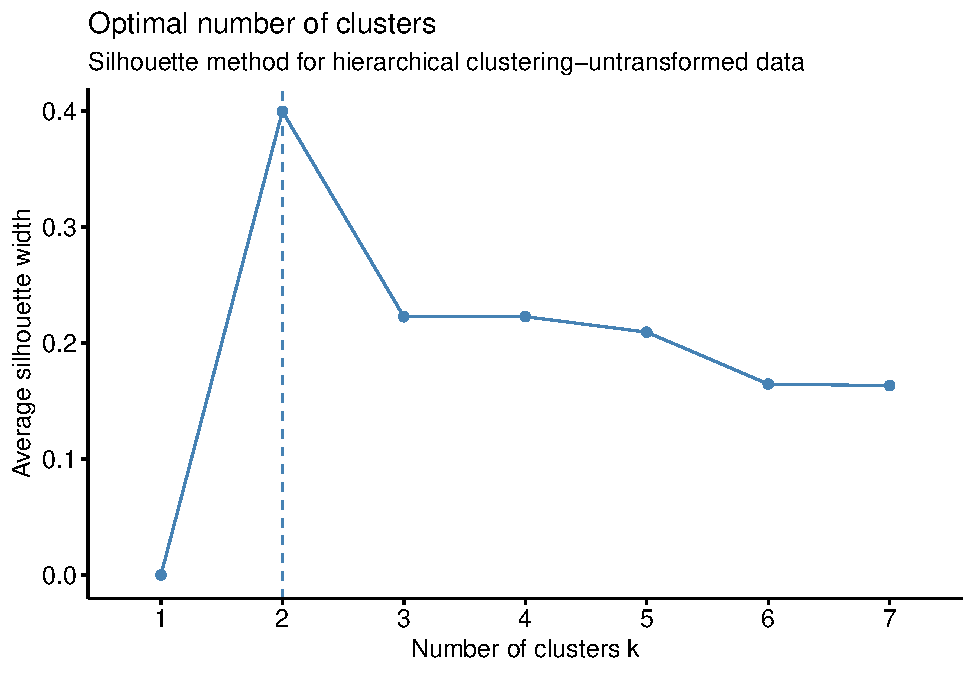
\includegraphics{week1_exercises_files/figure-latex/unnamed-chunk-6-1.pdf}

\begin{Shaded}
\begin{Highlighting}[]
\CommentTok{\#boxplot}
\FunctionTok{boxplot}\NormalTok{(genesDF[,}\DecValTok{1}\NormalTok{],}
     \AttributeTok{main =} \StringTok{"Boxplot of gene expressions"}\NormalTok{,}
     \AttributeTok{col =} \StringTok{"lightblue"}\NormalTok{, }\AttributeTok{border =} \StringTok{"black"}\NormalTok{)}
\end{Highlighting}
\end{Shaded}

\includegraphics{week1_exercises_files/figure-latex/unnamed-chunk-6-2.pdf}

\begin{enumerate}
\def\labelenumi{\arabic{enumi}.}
\setcounter{enumi}{1}
\tightlist
\item
  Test the difference of the means of the following simulated genes
  using the randomization, \texttt{t-test()} and \texttt{wilcox.test()}
  functions. Plot the distributions using histograms and boxplots.
  {[}Difficulty: \textbf{Intermediate/Advanced}{]}
\end{enumerate}

\begin{Shaded}
\begin{Highlighting}[]
\FunctionTok{set.seed}\NormalTok{(}\DecValTok{100}\NormalTok{)}
\NormalTok{gene1 }\OtherTok{=} \FunctionTok{rnorm}\NormalTok{(}\DecValTok{30}\NormalTok{, }\AttributeTok{mean =} \DecValTok{4}\NormalTok{, }\AttributeTok{sd =} \DecValTok{2}\NormalTok{)}
\NormalTok{gene2 }\OtherTok{=} \FunctionTok{rnorm}\NormalTok{(}\DecValTok{30}\NormalTok{, }\AttributeTok{mean =} \DecValTok{2}\NormalTok{, }\AttributeTok{sd =} \DecValTok{2}\NormalTok{)}
\CommentTok{\#calculate original difference}
\NormalTok{orig\_diff }\OtherTok{=} \FunctionTok{mean}\NormalTok{(gene1) }\SpecialCharTok{{-}} \FunctionTok{mean}\NormalTok{(gene2)}


\CommentTok{\#create a df for our data}
\NormalTok{genesDF }\OtherTok{=} \FunctionTok{data.frame}\NormalTok{(}\AttributeTok{exp =} \FunctionTok{c}\NormalTok{(gene1, gene2), }\AttributeTok{group =} \FunctionTok{c}\NormalTok{(}\FunctionTok{rep}\NormalTok{(}\StringTok{"group1"}\NormalTok{, }\DecValTok{30}\NormalTok{), }\FunctionTok{rep}\NormalTok{(}\StringTok{"group2"}\NormalTok{, }\DecValTok{30}\NormalTok{)))}
\CommentTok{\#null distribution{-}no difference in means }
\NormalTok{exp\_null }\OtherTok{\textless{}{-}} \FunctionTok{do}\NormalTok{(}\DecValTok{1000}\NormalTok{) }\SpecialCharTok{*} \FunctionTok{diff}\NormalTok{(mosaic}\SpecialCharTok{::}\FunctionTok{mean}\NormalTok{(exp }\SpecialCharTok{\textasciitilde{}} \FunctionTok{shuffle}\NormalTok{(group), }\AttributeTok{data =}\NormalTok{ genesDF))}

\CommentTok{\#test for differences using randomization}
\FunctionTok{hist}\NormalTok{(exp\_null[, }\DecValTok{1}\NormalTok{], }\AttributeTok{xlab =} \StringTok{"Null distribution | no difference in samples"}\NormalTok{,}
     \AttributeTok{main =} \FunctionTok{expression}\NormalTok{(}\FunctionTok{paste}\NormalTok{(H[}\DecValTok{0}\NormalTok{],}\StringTok{" :no difference in means"}\NormalTok{) ),}
     \AttributeTok{xlim =} \FunctionTok{c}\NormalTok{(}\SpecialCharTok{{-}}\DecValTok{2}\NormalTok{,}\DecValTok{2}\NormalTok{), }\AttributeTok{col =} \StringTok{"lightblue"}\NormalTok{, }\AttributeTok{border =} \StringTok{"white"}\NormalTok{)}
\FunctionTok{abline}\NormalTok{(}\AttributeTok{v =} \FunctionTok{quantile}\NormalTok{(exp\_null[, }\DecValTok{1}\NormalTok{], }\FloatTok{0.95}\NormalTok{), }\AttributeTok{col =} \StringTok{"black"}\NormalTok{)}
\FunctionTok{abline}\NormalTok{(}\AttributeTok{v =}\NormalTok{ orig\_diff, }\AttributeTok{col =} \StringTok{"red"}\NormalTok{ )}
\FunctionTok{text}\NormalTok{(}\AttributeTok{x =} \FunctionTok{quantile}\NormalTok{(exp\_null[, }\DecValTok{1}\NormalTok{], }\FloatTok{0.95}\NormalTok{), }\AttributeTok{y =} \DecValTok{200}\NormalTok{, }\StringTok{"0.05"}\NormalTok{, }\AttributeTok{adj =} \FunctionTok{c}\NormalTok{(}\DecValTok{1}\NormalTok{, }\DecValTok{0}\NormalTok{), }\AttributeTok{col =} \StringTok{"black"}\NormalTok{)}
\FunctionTok{text}\NormalTok{(}\AttributeTok{x =}\NormalTok{ orig\_diff, }\AttributeTok{y =} \DecValTok{250}\NormalTok{, }\StringTok{"orig\_diff."}\NormalTok{, }\AttributeTok{adj =} \FunctionTok{c}\NormalTok{(}\DecValTok{1}\NormalTok{, }\DecValTok{0}\NormalTok{), }\AttributeTok{col =} \StringTok{"red"}\NormalTok{)}
\end{Highlighting}
\end{Shaded}

\includegraphics{week1_exercises_files/figure-latex/exRnorm2chp3-1.pdf}

Test the difference of means of the simulated genes using
\texttt{t-test()}.

\begin{Shaded}
\begin{Highlighting}[]
\CommentTok{\#test differences of means using \textquotesingle{}t.test()\textquotesingle{}}
\NormalTok{stats}\SpecialCharTok{::}\FunctionTok{t.test}\NormalTok{(gene1, gene2)}
\end{Highlighting}
\end{Shaded}

\begin{verbatim}
## 
##  Welch Two Sample t-test
## 
## data:  gene1 and gene2
## t = 3.7653, df = 47.552, p-value = 0.0004575
## alternative hypothesis: true difference in means is not equal to 0
## 95 percent confidence interval:
##  0.872397 2.872761
## sample estimates:
## mean of x mean of y 
##  4.057728  2.185149
\end{verbatim}

Test the difference of means of the simulated genes using
\texttt{wilcox.test()}.

\begin{Shaded}
\begin{Highlighting}[]
\FunctionTok{wilcox.test}\NormalTok{(gene1, gene2, }\AttributeTok{conf.int =}\NormalTok{ T)}
\end{Highlighting}
\end{Shaded}

\begin{verbatim}
## 
##  Wilcoxon rank sum exact test
## 
## data:  gene1 and gene2
## W = 658, p-value = 0.001795
## alternative hypothesis: true location shift is not equal to 0
## 95 percent confidence interval:
##  0.6956318 2.7997818
## sample estimates:
## difference in location 
##               1.740907
\end{verbatim}

Plot the distributions using histograms and boxplots.

\begin{Shaded}
\begin{Highlighting}[]
\CommentTok{\#plot the distributions of gene expressions}
\FunctionTok{hist}\NormalTok{(genesDF[, }\DecValTok{1}\NormalTok{], }\CommentTok{\#histogram}
     \AttributeTok{main =} \StringTok{"Distribution of gene expressions"}\NormalTok{,}
     \AttributeTok{xlab =} \StringTok{"Gene expression"}\NormalTok{,}
     \AttributeTok{col =} \StringTok{"lightblue"}\NormalTok{, }\AttributeTok{border =} \StringTok{"white"}\NormalTok{)}
\end{Highlighting}
\end{Shaded}

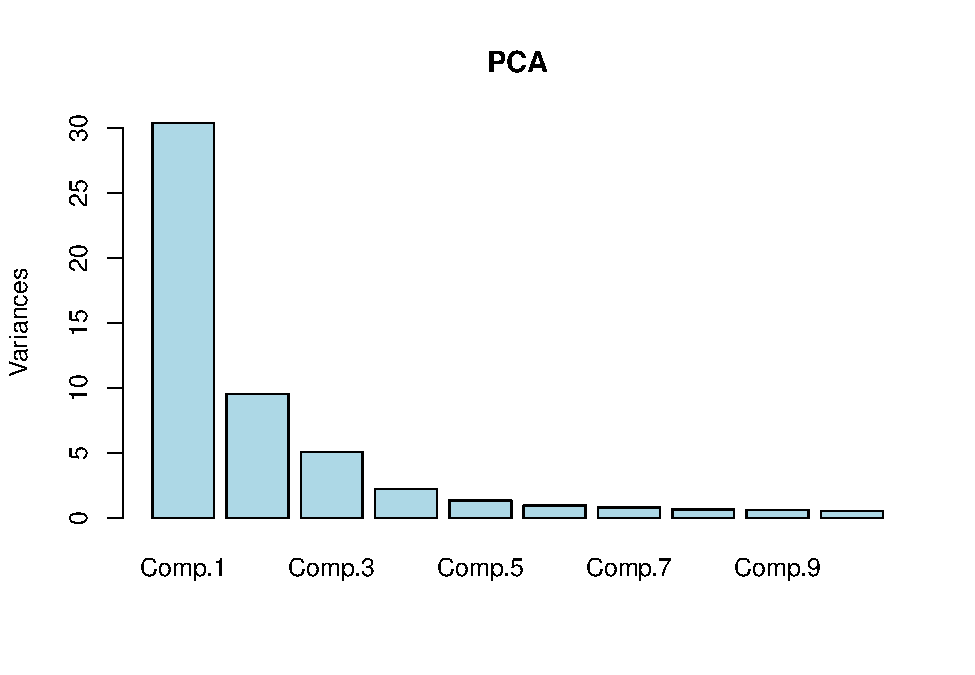
\includegraphics{week1_exercises_files/figure-latex/unnamed-chunk-9-1.pdf}

\begin{Shaded}
\begin{Highlighting}[]
\CommentTok{\#boxplot}
\FunctionTok{boxplot}\NormalTok{(genesDF[,}\DecValTok{1}\NormalTok{],}
     \AttributeTok{main =} \StringTok{"Boxplot of gene expressions"}\NormalTok{,}
     \AttributeTok{col =} \StringTok{"lightblue"}\NormalTok{, }\AttributeTok{border =} \StringTok{"black"}\NormalTok{)}
\end{Highlighting}
\end{Shaded}

\includegraphics{week1_exercises_files/figure-latex/unnamed-chunk-9-2.pdf}

\begin{enumerate}
\def\labelenumi{\arabic{enumi}.}
\setcounter{enumi}{2}
\tightlist
\item
  We need an extra data set for this exercise. Read the gene expression
  data set as follows:
  \texttt{gexpFile=system.file("extdata","geneExpMat.rds",package="compGenomRData")\ data=readRDS(gexpFile)}.
  The data has 100 differentially expressed genes. The first 3 columns
  are the test samples, and the last 3 are the control samples. Do a
  t-test for each gene (each row is a gene), and record the p-values.
  Then, do a moderated t-test, as shown in section ``Moderated t-tests''
  in this chapter, and record the p-values. Make a p-value histogram and
  compare two approaches in terms of the number of significant tests
  with the \(0.05\) threshold. On the p-values use FDR (BH), Bonferroni
  and q-value adjustment methods. Calculate how many adjusted p-values
  are below 0.05 for each approach. {[}Difficulty:
  \textbf{Intermediate/Advanced}{]}
\end{enumerate}

\begin{Shaded}
\begin{Highlighting}[]
\FunctionTok{require}\NormalTok{(matrixStats, }\AttributeTok{quietly =}\NormalTok{ T)}
\end{Highlighting}
\end{Shaded}

\begin{verbatim}
## 
## Attaching package: 'matrixStats'
\end{verbatim}

\begin{verbatim}
## The following objects are masked from 'package:mosaic':
## 
##     count, iqr
\end{verbatim}

\begin{verbatim}
## The following object is masked from 'package:dplyr':
## 
##     count
\end{verbatim}

\begin{Shaded}
\begin{Highlighting}[]
\CommentTok{\#import data}
\NormalTok{gexpFile }\OtherTok{=} \FunctionTok{system.file}\NormalTok{(}\StringTok{"extdata"}\NormalTok{, }\StringTok{"geneExpMat.rds"}\NormalTok{, }\AttributeTok{package =} \StringTok{"compGenomRData"}\NormalTok{) }
\NormalTok{data }\OtherTok{=} \FunctionTok{readRDS}\NormalTok{(gexpFile)}

\CommentTok{\#true difference in means}
\NormalTok{dx }\OtherTok{=} \FunctionTok{rowMeans}\NormalTok{(data[, }\DecValTok{1}\SpecialCharTok{:}\DecValTok{3}\NormalTok{]) }\SpecialCharTok{{-}} \FunctionTok{rowMeans}\NormalTok{(data[, }\DecValTok{4}\SpecialCharTok{:}\DecValTok{6}\NormalTok{])}

\NormalTok{n1 }\OtherTok{=} \DecValTok{3}
\NormalTok{n2 }\OtherTok{=} \DecValTok{3}
\CommentTok{\#get the esimate of pooled variance }
\NormalTok{stderr }\OtherTok{=} \FunctionTok{sqrt}\NormalTok{((}\FunctionTok{rowVars}\NormalTok{(data[, }\DecValTok{1}\SpecialCharTok{:}\DecValTok{3}\NormalTok{])}\SpecialCharTok{*}\NormalTok{(n1}\DecValTok{{-}1}\NormalTok{) }\SpecialCharTok{+} \FunctionTok{rowVars}\NormalTok{(data[, }\DecValTok{4}\SpecialCharTok{:}\DecValTok{6}\NormalTok{])}\SpecialCharTok{*}\NormalTok{(n2}\DecValTok{{-}1}\NormalTok{)) }\SpecialCharTok{/}\NormalTok{ (n1}\SpecialCharTok{+}\NormalTok{n2}\DecValTok{{-}2}\NormalTok{) }\SpecialCharTok{*}\NormalTok{ ( }\DecValTok{1}\SpecialCharTok{/}\NormalTok{n1 }\SpecialCharTok{+} \DecValTok{1}\SpecialCharTok{/}\NormalTok{n2 ))}
\CommentTok{\#do the shrinking towards median}
\NormalTok{mod.stderr }\OtherTok{=}\NormalTok{ (stderr }\SpecialCharTok{+} \FunctionTok{median}\NormalTok{(stderr)) }\SpecialCharTok{/} \DecValTok{2} \CommentTok{\# moderation in variation}

\CommentTok{\#do a t{-}test for each gene and record p{-}values}
\NormalTok{t }\OtherTok{=}\NormalTok{ dx }\SpecialCharTok{/}\NormalTok{ stderr}
\NormalTok{p }\OtherTok{=} \DecValTok{2}\SpecialCharTok{*}\FunctionTok{pt}\NormalTok{( }\SpecialCharTok{{-}}\FunctionTok{abs}\NormalTok{(t), n1}\SpecialCharTok{+}\NormalTok{n2}\DecValTok{{-}2}\NormalTok{ )}

\CommentTok{\#do a moderated t{-}test and record p{-}values}
\NormalTok{t.mod }\OtherTok{\textless{}{-}}\NormalTok{ dx }\SpecialCharTok{/}\NormalTok{ mod.stderr}
\NormalTok{p.mod }\OtherTok{=} \DecValTok{2}\SpecialCharTok{*}\FunctionTok{pt}\NormalTok{( }\SpecialCharTok{{-}}\FunctionTok{abs}\NormalTok{(t.mod), n1}\SpecialCharTok{+}\NormalTok{n2}\DecValTok{{-}2}\NormalTok{ )}

\CommentTok{\#make a p{-}value histogram and compare both approaches}
\FunctionTok{par}\NormalTok{(}\AttributeTok{mfrow =} \FunctionTok{c}\NormalTok{(}\DecValTok{1}\NormalTok{, }\DecValTok{2}\NormalTok{))}

\FunctionTok{hist}\NormalTok{(p, }\AttributeTok{col =} \StringTok{"lightblue"}\NormalTok{, }\AttributeTok{border =} \StringTok{"white"}\NormalTok{, }\AttributeTok{main =} \StringTok{""}\NormalTok{,}
     \AttributeTok{xlab =} \StringTok{"P{-}values t{-}test"}\NormalTok{)}
\FunctionTok{mtext}\NormalTok{(}\FunctionTok{paste}\NormalTok{(}\StringTok{"Signifcant tests:"}\NormalTok{, }\FunctionTok{sum}\NormalTok{(p }\SpecialCharTok{\textless{}} \FloatTok{0.05}\NormalTok{))  )}

\FunctionTok{hist}\NormalTok{(p.mod, }\AttributeTok{col =} \StringTok{"lightblue"}\NormalTok{, }\AttributeTok{border=}\StringTok{"white"}\NormalTok{, }\AttributeTok{main=}\StringTok{""}\NormalTok{,}
     \AttributeTok{xlab=}\StringTok{"P{-}values mod. t{-}test"}\NormalTok{)}
\FunctionTok{mtext}\NormalTok{(}\FunctionTok{paste}\NormalTok{(}\StringTok{"Signifcant tests:"}\NormalTok{, }\FunctionTok{sum}\NormalTok{(p.mod }\SpecialCharTok{\textless{}}\FloatTok{0.05}\NormalTok{)))}
\end{Highlighting}
\end{Shaded}

\includegraphics{week1_exercises_files/figure-latex/unnamed-chunk-10-1.pdf}

On the p-values use FDR (BH), Bonferroni and q-value adjustment methods.
Calculate how many adjusted p-values are below 0.05 for each approach.

\begin{Shaded}
\begin{Highlighting}[]
\FunctionTok{require}\NormalTok{(qvalue, }\AttributeTok{quietly =}\NormalTok{ T)}

\CommentTok{\#FDR adjusted value}
\NormalTok{fdr.adj.pval }\OtherTok{=} \FunctionTok{p.adjust}\NormalTok{(p, }\AttributeTok{method =} \StringTok{"fdr"}\NormalTok{)}
\CommentTok{\#Bonferroni correction}
\NormalTok{bonf.pval}\OtherTok{=}\FunctionTok{p.adjust}\NormalTok{(p, }\AttributeTok{method =} \StringTok{"bonferroni"}\NormalTok{)}
\CommentTok{\#q{-}value}
\NormalTok{qvalues }\OtherTok{\textless{}{-}} \FunctionTok{qvalue}\NormalTok{(p)}\SpecialCharTok{$}\NormalTok{q}

\NormalTok{n\_pvalues }\OtherTok{\textless{}{-}} \FunctionTok{data.frame}\NormalTok{(}\AttributeTok{fdr\_adj\_pval =} \FunctionTok{c}\NormalTok{(}\FunctionTok{sum}\NormalTok{(fdr.adj.pval }\SpecialCharTok{\textless{}} \FloatTok{0.05}\NormalTok{)),}
                        \AttributeTok{bonf\_pval =} \FunctionTok{sum}\NormalTok{(bonf.pval }\SpecialCharTok{\textless{}} \FloatTok{0.05}\NormalTok{),}
                        \AttributeTok{q\_values =} \FunctionTok{sum}\NormalTok{(qvalues }\SpecialCharTok{\textless{}} \FloatTok{0.05}\NormalTok{))}
\FunctionTok{rownames}\NormalTok{(n\_pvalues) }\OtherTok{\textless{}{-}} \StringTok{"\# of p{-}values below 0.05"}
\NormalTok{n\_pvalues}
\end{Highlighting}
\end{Shaded}

\begin{verbatim}
##                          fdr_adj_pval bonf_pval q_values
## # of p-values below 0.05           99        25      100
\end{verbatim}

\hypertarget{relationship-between-variables-linear-models-and-correlation}{%
\subsubsection{Relationship between variables: Linear models and
correlation}\label{relationship-between-variables-linear-models-and-correlation}}

Below we are going to simulate X and Y values that are needed for the
rest of the exercise.

\begin{Shaded}
\begin{Highlighting}[]
\CommentTok{\# set random number seed, so that the random numbers from the text}
\CommentTok{\# is the same when you run the code.}
\FunctionTok{set.seed}\NormalTok{(}\DecValTok{32}\NormalTok{)}

\CommentTok{\# get 50 X values between 1 and 100}
\NormalTok{x }\OtherTok{=} \FunctionTok{runif}\NormalTok{(}\DecValTok{50}\NormalTok{, }\DecValTok{1}\NormalTok{, }\DecValTok{100}\NormalTok{)}

\CommentTok{\# set b0,b1 and variance (sigma)}
\NormalTok{b0 }\OtherTok{=} \DecValTok{10}
\NormalTok{b1 }\OtherTok{=} \DecValTok{2}
\NormalTok{sigma }\OtherTok{=} \DecValTok{20}
\CommentTok{\# simulate error terms from normal distribution}
\NormalTok{eps }\OtherTok{=} \FunctionTok{rnorm}\NormalTok{(}\DecValTok{50}\NormalTok{, }\DecValTok{0}\NormalTok{, sigma)}
\CommentTok{\# get y values from the linear equation and addition of error terms}
\NormalTok{y }\OtherTok{=}\NormalTok{ b0 }\SpecialCharTok{+}\NormalTok{ b1}\SpecialCharTok{*}\NormalTok{x}\SpecialCharTok{+}\NormalTok{ eps}
\end{Highlighting}
\end{Shaded}

\begin{enumerate}
\def\labelenumi{\arabic{enumi}.}
\tightlist
\item
  Run the code then fit a line to predict Y based on X.
  {[}Difficulty:\textbf{Intermediate}{]}
\end{enumerate}

\begin{Shaded}
\begin{Highlighting}[]
\CommentTok{\#instance the model}
\NormalTok{model }\OtherTok{\textless{}{-}} \FunctionTok{lm}\NormalTok{(y }\SpecialCharTok{\textasciitilde{}}\NormalTok{ x)}
\end{Highlighting}
\end{Shaded}

\begin{enumerate}
\def\labelenumi{\arabic{enumi}.}
\setcounter{enumi}{1}
\tightlist
\item
  Plot the scatter plot and the fitted line.
  {[}Difficulty:\textbf{Intermediate}{]}
\end{enumerate}

\begin{Shaded}
\begin{Highlighting}[]
\CommentTok{\#scatter plot}
\FunctionTok{plot}\NormalTok{(x, y, }\AttributeTok{pch=}\DecValTok{20}\NormalTok{)}
\CommentTok{\#plot the fitted line}
\FunctionTok{abline}\NormalTok{(model, }\AttributeTok{col =} \StringTok{"red"}\NormalTok{)}
\end{Highlighting}
\end{Shaded}

\includegraphics{week1_exercises_files/figure-latex/unnamed-chunk-13-1.pdf}

\begin{enumerate}
\def\labelenumi{\arabic{enumi}.}
\setcounter{enumi}{2}
\tightlist
\item
  Calculate correlation and R\^{}2.
  {[}Difficulty:\textbf{Intermediate}{]}
\end{enumerate}

\begin{Shaded}
\begin{Highlighting}[]
\FunctionTok{cat}\NormalTok{(}\StringTok{"Correlation of model: "}\NormalTok{, correlation }\OtherTok{\textless{}{-}} \FunctionTok{cor}\NormalTok{(x, y), }\StringTok{"}\SpecialCharTok{\textbackslash{}n}\StringTok{"}\NormalTok{)}
\end{Highlighting}
\end{Shaded}

\begin{verbatim}
## Correlation of model:  0.9511939
\end{verbatim}

\begin{Shaded}
\begin{Highlighting}[]
\NormalTok{R2 }\OtherTok{\textless{}{-}}\FunctionTok{summary.lm}\NormalTok{(model)}\SpecialCharTok{$}\NormalTok{r.squared}
\FunctionTok{cat}\NormalTok{(}\StringTok{"R squared of model: "}\NormalTok{, R2)}
\end{Highlighting}
\end{Shaded}

\begin{verbatim}
## R squared of model:  0.9047699
\end{verbatim}

Correlation shows a high value of correlation between both variables.
The R\^{}2 is sufficiently good to assume that the `x' variable has the
power to predict `y' values.

\begin{enumerate}
\def\labelenumi{\arabic{enumi}.}
\setcounter{enumi}{3}
\tightlist
\item
  Run the \texttt{summary()} function and try to extract P-values for
  the model from the object returned by \texttt{summary}. See
  \texttt{?summary.lm}. {[}Difficulty:\textbf{Intermediate/Advanced}{]}
\end{enumerate}

\begin{Shaded}
\begin{Highlighting}[]
\CommentTok{\#p{-}value: \textless{} 2.2e{-}16}
\NormalTok{sum }\OtherTok{\textless{}{-}} \FunctionTok{summary.lm}\NormalTok{(model)}
\NormalTok{sum}
\end{Highlighting}
\end{Shaded}

\begin{verbatim}
## 
## Call:
## lm(formula = y ~ x)
## 
## Residuals:
##    Min     1Q Median     3Q    Max 
## -38.50 -12.62   1.66  14.26  37.20 
## 
## Coefficients:
##             Estimate Std. Error t value Pr(>|t|)    
## (Intercept)  0.40951    6.43208   0.064     0.95    
## x            2.08742    0.09775  21.355   <2e-16 ***
## ---
## Signif. codes:  0 '***' 0.001 '**' 0.01 '*' 0.05 '.' 0.1 ' ' 1
## 
## Residual standard error: 16.96 on 48 degrees of freedom
## Multiple R-squared:  0.9048, Adjusted R-squared:  0.9028 
## F-statistic:   456 on 1 and 48 DF,  p-value: < 2.2e-16
\end{verbatim}

\begin{enumerate}
\def\labelenumi{\arabic{enumi}.}
\setcounter{enumi}{4}
\tightlist
\item
  Plot the residuals vs.~the fitted values plot, by calling the
  \texttt{plot()} function with \texttt{which=1} as the second argument.
  First argument is the model returned by \texttt{lm()}.
  {[}Difficulty:\textbf{Advanced}{]}
\end{enumerate}

\begin{Shaded}
\begin{Highlighting}[]
\FunctionTok{plot}\NormalTok{(model, }\AttributeTok{which =} \DecValTok{1}\NormalTok{)}
\end{Highlighting}
\end{Shaded}

\includegraphics{week1_exercises_files/figure-latex/unnamed-chunk-16-1.pdf}

The plot above shows no obvious pattern between our residuals and fitted
values, showing no tendecy in our model.

\begin{enumerate}
\def\labelenumi{\arabic{enumi}.}
\setcounter{enumi}{5}
\tightlist
\item
  For the next exercises, read the data set histone modification data
  set. Use the following to get the path to the file:
\end{enumerate}

\begin{Shaded}
\begin{Highlighting}[]
\CommentTok{\#import data}
\NormalTok{hmodFile}\OtherTok{=}\FunctionTok{system.file}\NormalTok{(}\StringTok{"extdata"}\NormalTok{,}
                    \StringTok{"HistoneModeVSgeneExp.rds"}\NormalTok{,}
                     \AttributeTok{package=}\StringTok{"compGenomRData"}\NormalTok{)}
\NormalTok{data2 }\OtherTok{\textless{}{-}} \FunctionTok{readRDS}\NormalTok{(hmodFile)}
\end{Highlighting}
\end{Shaded}

There are 3 columns in the dataset. These are measured levels of
H3K4me3, H3K27me3 and gene expression per gene. Once you read in the
data, plot the scatter plot for H3K4me3 vs.~expression.
{[}Difficulty:\textbf{Beginner}{]}

\begin{Shaded}
\begin{Highlighting}[]
\FunctionTok{library}\NormalTok{(ggplot2)}

\CommentTok{\#plot H3K4me3 vs. expression.}
\FunctionTok{ggplot}\NormalTok{(data2, }\FunctionTok{aes}\NormalTok{(}\AttributeTok{x =}\NormalTok{ H3k4me3, }\AttributeTok{y =}\NormalTok{ measured\_log2)) }\SpecialCharTok{+} 
  \FunctionTok{geom\_point}\NormalTok{()}
\end{Highlighting}
\end{Shaded}

\includegraphics{week1_exercises_files/figure-latex/unnamed-chunk-18-1.pdf}

\begin{enumerate}
\def\labelenumi{\arabic{enumi}.}
\setcounter{enumi}{6}
\tightlist
\item
  Plot the scatter plot for H3K27me3 vs.~expression.
  {[}Difficulty:\textbf{Beginner}{]}
\end{enumerate}

\begin{Shaded}
\begin{Highlighting}[]
\CommentTok{\#plot H3K27me3 vs. expression}
\FunctionTok{ggplot}\NormalTok{(data2, }\FunctionTok{aes}\NormalTok{(}\AttributeTok{x =}\NormalTok{ H3k27me3, }\AttributeTok{y =}\NormalTok{ measured\_log2)) }\SpecialCharTok{+} 
  \FunctionTok{geom\_point}\NormalTok{()}
\end{Highlighting}
\end{Shaded}

\includegraphics{week1_exercises_files/figure-latex/unnamed-chunk-19-1.pdf}

\begin{enumerate}
\def\labelenumi{\arabic{enumi}.}
\setcounter{enumi}{7}
\tightlist
\item
  Fit the model for prediction of expression data using: 1) Only H3K4me3
  as explanatory variable, 2) Only H3K27me3 as explanatory variable, and
  3) Using both H3K4me3 and H3K27me3 as explanatory variables. Inspect
  the \texttt{summary()} function output in each case, which terms are
  significant. {[}Difficulty:\textbf{Beginner/Intermediate}{]}
\end{enumerate}

\begin{enumerate}
\def\labelenumi{\arabic{enumi})}
\tightlist
\item
\end{enumerate}

\begin{Shaded}
\begin{Highlighting}[]
\CommentTok{\#fitting a regression model using H3K4me3 as explanatory variable}
\NormalTok{model2 }\OtherTok{\textless{}{-}} \FunctionTok{lm}\NormalTok{(measured\_log2 }\SpecialCharTok{\textasciitilde{}}\NormalTok{ H3k4me3, }\AttributeTok{data =}\NormalTok{ data2)}
\FunctionTok{summary}\NormalTok{(model2)}
\end{Highlighting}
\end{Shaded}

\begin{verbatim}
## 
## Call:
## lm(formula = measured_log2 ~ H3k4me3, data = data2)
## 
## Residuals:
##      Min       1Q   Median       3Q      Max 
## -11.0503  -1.0218  -0.1054   1.2508  11.2229 
## 
## Coefficients:
##             Estimate Std. Error t value Pr(>|t|)    
## (Intercept) -9.68153    0.05853  -165.4   <2e-16 ***
## H3k4me3      2.33263    0.01457   160.1   <2e-16 ***
## ---
## Signif. codes:  0 '***' 0.001 '**' 0.01 '*' 0.05 '.' 0.1 ' ' 1
## 
## Residual standard error: 2.565 on 13729 degrees of freedom
## Multiple R-squared:  0.6511, Adjusted R-squared:  0.6511 
## F-statistic: 2.563e+04 on 1 and 13729 DF,  p-value: < 2.2e-16
\end{verbatim}

From the above output, the first thing to notice is the p-value of the
model, which is close to 0, meaning that we can trust the model. As so,
p-values for the explanatory variable `H3K4me3' and for the intercept
are really trustworthy.

\begin{enumerate}
\def\labelenumi{\arabic{enumi})}
\setcounter{enumi}{1}
\tightlist
\item
\end{enumerate}

\begin{Shaded}
\begin{Highlighting}[]
\CommentTok{\#fitting a regression model using H3K27me3 as explanatory variable}
\NormalTok{model3 }\OtherTok{\textless{}{-}} \FunctionTok{lm}\NormalTok{(measured\_log2 }\SpecialCharTok{\textasciitilde{}}\NormalTok{ H3k27me3, }\AttributeTok{data =}\NormalTok{ data2)}
\FunctionTok{summary}\NormalTok{(model3)}
\end{Highlighting}
\end{Shaded}

\begin{verbatim}
## 
## Call:
## lm(formula = measured_log2 ~ H3k27me3, data = data2)
## 
## Residuals:
##     Min      1Q  Median      3Q     Max 
## -4.8885 -4.0716 -0.5573  3.8014 12.9216 
## 
## Coefficients:
##             Estimate Std. Error t value Pr(>|t|)    
## (Intercept) -0.36390    0.04394  -8.282   <2e-16 ***
## H3k27me3    -0.78807    0.03117 -25.283   <2e-16 ***
## ---
## Signif. codes:  0 '***' 0.001 '**' 0.01 '*' 0.05 '.' 0.1 ' ' 1
## 
## Residual standard error: 4.245 on 13729 degrees of freedom
## Multiple R-squared:  0.04449,    Adjusted R-squared:  0.04442 
## F-statistic: 639.2 on 1 and 13729 DF,  p-value: < 2.2e-16
\end{verbatim}

Our second model, has the same p-values for the explanatory variable
`H3K27me3', intercept and overall model. Nevertheless, it's R-squared
score is less significant that the score of our previous model (0.04449
\textless{} 0.6511), which indicates that the correlation between
`H3K27me3' and gene expression `measured\_log2' is stronger than
`H3K27me3' and gene expression. 3)

\begin{Shaded}
\begin{Highlighting}[]
\CommentTok{\#fitting a regression model using both epigenetic marks as explanatory variables}
\NormalTok{model4 }\OtherTok{\textless{}{-}} \FunctionTok{lm}\NormalTok{(measured\_log2 }\SpecialCharTok{\textasciitilde{}}\NormalTok{ H3k4me3 }\SpecialCharTok{+}\NormalTok{ H3k27me3, }\AttributeTok{data =}\NormalTok{ data2)}
\FunctionTok{summary}\NormalTok{(model4)}
\end{Highlighting}
\end{Shaded}

\begin{verbatim}
## 
## Call:
## lm(formula = measured_log2 ~ H3k4me3 + H3k27me3, data = data2)
## 
## Residuals:
##      Min       1Q   Median       3Q      Max 
## -11.0564  -1.0702  -0.3066   1.2486  10.8950 
## 
## Coefficients:
##             Estimate Std. Error t value Pr(>|t|)    
## (Intercept) -9.11803    0.05980 -152.48   <2e-16 ***
## H3k4me3      2.29815    0.01417  162.17   <2e-16 ***
## H3k27me3    -0.54532    0.01832  -29.77   <2e-16 ***
## ---
## Signif. codes:  0 '***' 0.001 '**' 0.01 '*' 0.05 '.' 0.1 ' ' 1
## 
## Residual standard error: 2.486 on 13728 degrees of freedom
## Multiple R-squared:  0.6723, Adjusted R-squared:  0.6723 
## F-statistic: 1.408e+04 on 2 and 13728 DF,  p-value: < 2.2e-16
\end{verbatim}

Our multivariate model shows to be a better model that the models using
a single explanatory variable, with a R-squared score = 0.6723. Which
suggests that predicting gene expression is better when both epigenetic
marks are used in modeling.

\begin{enumerate}
\def\labelenumi{\arabic{enumi}.}
\setcounter{enumi}{9}
\tightlist
\item
  Is using H3K4me3 and H3K27me3 better than the model with only H3K4me3?
  {[}Difficulty:\textbf{Intermediate}{]}
\end{enumerate}

Both summary statistics shows that both models are competent in
predicting gene expression. For a better answer, let's compare the
correlation coefficient.

\begin{Shaded}
\begin{Highlighting}[]
\NormalTok{singlemodelCorr }\OtherTok{\textless{}{-}} \FunctionTok{summary.lm}\NormalTok{(model2)}\SpecialCharTok{$}\NormalTok{r.squared}
\NormalTok{multimodelCorr }\OtherTok{\textless{}{-}} \FunctionTok{summary.lm}\NormalTok{(model4)}\SpecialCharTok{$}\NormalTok{r.squared}

\FunctionTok{cat}\NormalTok{(}\StringTok{"Correlation of model with only H3K4me3 as explanatory variable: "}\NormalTok{, singlemodelCorr, }\StringTok{"}\SpecialCharTok{\textbackslash{}n}\StringTok{"}\NormalTok{)}
\end{Highlighting}
\end{Shaded}

\begin{verbatim}
## Correlation of model with only H3K4me3 as explanatory variable:  0.6511409
\end{verbatim}

\begin{Shaded}
\begin{Highlighting}[]
\FunctionTok{cat}\NormalTok{(}\StringTok{"Correlation of model with H3K4me3 and H3K27me3 as explanatory variables: "}\NormalTok{, multimodelCorr)}
\end{Highlighting}
\end{Shaded}

\begin{verbatim}
## Correlation of model with H3K4me3 and H3K27me3 as explanatory variables:  0.6722997
\end{verbatim}

We can appreciate a slight increase in the correlation coefficient of
the model that uses both epigenetic marks, so we can conclude that this
model is better than the model using just H3K4me3.

\end{document}
